%%Modified
%%
%% This is file `cescgsmpl.tex',
%% generated with the docstrip utility.
%%
%% The original source files were:
%%
%% cescg.dtx  (with options: `sample')
%% 
%% IMPORTANT NOTICE:
%% 
%% For the copyright see the source file.
%% 
%% Any modified versions of this file must be renamed
%% with new filenames distinct from cescgsmpl.tex.
%% 
%% For distribution of the original source see the terms
%% for copying and modification in the file cescg.dtx.
%% 
%% This generated file may be distributed as long as the
%% original source files, as listed above, are part of the
%% same distribution. (The sources need not necessarily be
%% in the same archive or directory.)
%% Copyright (c) 1999, 2005
%%               Institute of Computer Graphics and Algorithms
%%               TU Vienna, Austria
%% Based on the LaTeX2e document class SCCG
%% Copyright (C) 1999 Pavel Chalmoviansky
%%                    Katedra geometrie
%%                    Faculty of Mathematics and Physics
%%                    Comenius University, Bratislava
%%                    chalmo@fmph.uniba.sk
%%
%% This file is distributed in the hope that it will be useful,
%% but WITHOUT ANY WARRANTY; without even the implied warranty of
%% MERCHANTABILITY or FITNESS FOR A PARTICULAR PURPOSE.
%%
%% \CharacterTable
%%  {Upper-case    \A\B\C\D\E\F\G\H\I\J\K\L\M\N\O\P\Q\R\S\T\U\V\W\X\Y\Z
%%   Lower-case    \a\b\c\d\e\f\g\h\i\j\k\l\m\n\o\p\q\r\s\t\u\v\w\x\y\z
%%   Digits        \0\1\2\3\4\5\6\7\8\9
%%   Exclamation   \!     Double quote  \"     Hash (number) \#
%%   Dollar        \$     Percent       \%     Ampersand     \&
%%   Acute accent  \'     Left paren    \(     Right paren   \)
%%   Asterisk      \*     Plus          \+     Comma         \,
%%   Minus         \-     Point         \.     Solidus       \/
%%   Colon         \:     Semicolon     \;     Less than     \<
%%   Equals        \=     Greater than  \>     Question mark \?
%%   Commercial at \@     Left bracket  \[     Backslash     \\
%%   Right bracket \]     Circumflex    \^     Underscore    \_
%%   Grave accent  \`     Left brace    \{     Vertical bar  \|
%%   Right brace   \}     Tilde         \~}
%%
\ProvidesFile{cescgsmpl.tex}
            [2005/11/29 v0.1.4
 CESCG proceedings sample file]
 %%% The document class command loads the CESCG class and sets the basic
 %%%  options.  See the user's guide for more options and their meaning.


\documentclass{cescg}[2005/11/12] % Use this for your submission and the final paper
 %%% Use e.g. this package to include figures via \includegraphics[options]{filename}.
 %%% If you don't have it in your latex installation, complain to your
 %%% sysadmin that he's not doing his job.
\usepackage{graphicx}
\usepackage{amsmath}
\usepackage{array}
\usepackage{url}
 %%% The following packages are somewhat system and installation dependent, and may not work
 %%% on some systems.
 %%% If you use pdfLaTeX on Windows (part of MiKTeX), you may use package epstopdf to automatically
 %%% convert eps files to pdf. Use this line:
 %\usepackage{epstopdf}
 %%% Linux users may have to call epstopdf on the command line or configure a Makefile appropriately.

 %%% If you know how to create bounding boxes for png and jpg files, you can uncomment this
 %%% to include png files etc. directly.
 %%% For example bmeps -b myfigure.png >myfigure.bb will do the trick in Windows.
 %%% Also, dvips needs the option "-I c3r8f" to be able to convert the bitmaps.
 %%% See the bmeps faq for more info: http://bmeps.sourceforge.net/faq.html
 %\ifx\pdfoutput\undefined \DeclareGraphicsExtensions{.eps,.png,.gif,.jpg} \fi

 %%% Now we set the fields for the title block and cover sheet
 %%% See the user's guide for more information on these items

 %% Title, author(s), and affiliation
 %%  Note that we have included both individual affiliations for each author
 %%   within the author block, as well as a common affiliation.  Only one
 %%   of these is necessary.
 %%  Footnotes to items in the title block should be created with the \thanks
 %%   command.
\title{Real-Time Rigid Body Simulation with Constraints}

 %%The first submission (for reviewing) must be annonymous due to the double-blind reviewing process. There must be no personal and no affiliation details of the authors.
%\author{Paper06}
 %Uncomment these for the camera-ready version
 \author{Zolt\'an Jakab\thanks{zolija@freemail.hu} }
 \supervisor{L\'aszl\'o Sz\'ecsi\thanks{szecsi@iit.bme.hu}}
 \affiliation{Department of Control Engineering and Information Technology\\
              Budapest University of Technology and Economics\\
              Budapest~/~Hungary}

 %% Keywords of paper
\keywords{Physical Simulation, Collision Detection, Rigid Bodies}
 %%% Begin the paper
\begin{document}

 %%% Create the title block
\maketitle

 %%% The abstract
\begin{abstract}
Rigid body simulation with constraints offers a well-established and robust approach to a wide range of physical phenomena, offering great flexibility by allowing custom constraints. This includes elastic or plastic simulations more commonly handled by mass-spring systems or position-based dynamics. In this paper, we present a simple but functional real-time physics simulation based on rigid body dynamics with pre-defined and contact constraints, and explore its applicability in cloth, hair, and ragdoll simulation. We compare our results against those achieved with position-based dynamics.
\end{abstract}

 %%% Keywords

\keywordlist

\section{Introduction}
When a high number of rigid bodies are connected using constraints, we obtain dynamic systems akin to discretized deformable bodies like ropes, hair, or cloth. While performing the simulation of such systems using rigid body dynamics is an expensive approach, it inherently provides solutions for collisions, friction, or inextendibility. In this paper, we describe a rigid body simulation framework that supports constraints necessary for approximating deformable bodies, and we evaluate the performance and stability against an implementation of  the most often used position-based dynamics~\cite{muller2007position} approach.
%We compare our method of using connected rigid bodies for hair and cloth simulation against this baseline, and identify cases where our approach may have benefits.
%??? I think about big braids of hair colliding with one another. Simple fixed constraints like hairbands are well handled by position-based dynamics (PBD).
We also implement character animation, where jointed rigid bodies are already the state of the art.

\section{Previous work}

The motion of rigid bodies can be modeled using Lagrangian mechanics. This framework allows us to use both forces and constraints to control the motion of bodies. Placing constraints on the velocities of objects can prevent the simulation from transitioning into invalid position states, enabling the creation of stiff systems. However, solving these constraints takes a significant amount of calculation, and the stiffness often causes instabilities.

An alternative, used by PBD~\cite{muller2007position}, is to only use positions in calculations. Velocities are computed from the displacements in the previous time step, adding the effect of external forces. Positions for the next iteration are first computed by forward Euler integration, and then constraints are applied to them sequentially an iteratively, making adjustments along the constraint function gradients one-at-a-time. This is more stable, but does not directly support rotation constraints, and constraints are characteristically elastic.

Real-time hair simulation is generally based on the work of Müller et al.~\cite{muller2012fast}, supporting highly dynamic simulation of a high number of inextensible hair strands, but without interaction between hair strands handled only through a density field. 

For hair simulation, working with large numbers of strands has become increasingly popular. Some specialized algorithms are capable of simulating each strand of hair individually, whereas with rigid bodies, only a lower number of guide strands can be simulated, since each body requires a relatively large number of calculations. In the video game industry, real-time performance, and artist control over simulations is important. For this reason, it is common to reuse existing skeletal animation and rigid body simulation systems to control hair guide strands through chains of bones~\cite{rungjiratananon2015physics}. The low resource consumption of this method makes it suitable for lower-end (such as mobile) devices, or as part of a LoD scheme even if more expensive methods are used for characters close to the camera.

\section{Lagrange's equations}
In three dimensional space, the position of a rigid body can be described with three Cartesian coordinates, and its rotation with three Euler angles (or an equivalent rotation representation, such as quaternions). Thus, given \(N\) independent bodies, we can describe them with \(6N\) coordinates. These are called maximal coordinates. To enforce constraints, Lagrange multipliers are used, giving equations of the following kind (Lagrange's equations):
\[\frac{\partial L}{\partial r_k}-\frac{d}{dt}\frac{\partial L}{\partial \dot{r_k}}+\sum_i \lambda_i \frac{\partial f_i}{\partial r_k} = 0\]
where \(L\) is the Lagrangian, which describes the total energy of the system in terms of the positions (linear and angular) \(r_k\) and velocities \(\dot{r_k}\) of the rigid bodies, \(f_i\) are constraint functions, which depend on the positions of rigid bodies and have to evaluate to zero in valid configurations, and \(\lambda_i\) are the Lagrange multipliers.
An alternative to this is the use of reduced coordinates, which are selected such that all combinations of coordinates yield valid configurations. This simplifies Lagrange's equations to:
\[\frac{d}{dt}\frac{\partial L}{\partial \dot{q_k}}=\frac{\partial L}{\partial q_k}\]
Unfortunately, except for the simplest cases, it is difficult to find such coordinate systems.

Most physics engines use maximal coordinates, because they are more flexible in their use, but some allow the use of Featherstone’s algorithm for tree-like kinematic chains~\cite{coumans2014exploring}. In this limited case, using reduced coordinates is feasible and can be more efficient. We have found that using maximal coordinates provides adequate results for most common systems, and have not pursued reduced coordinate methods further for now.

Lagrange’s equations can be solved using the following general method:
\begin{itemize}
\item Calculate the forces and constraints that affect the bodies. This can depend on the state of the system (that is the positions, velocities, and time).
\item Apply an integrator to calculate the new state, and repeat.
\end{itemize}
The most important properties of an integrator are its accuracy, stability and computational efficiency. Accuracy is usually measured by the order of a method (an integrator has order p if its global error scales as \(O(h^p)\) where \(h\) is the time step). For real-time simulations, where inaccuracy is acceptable, it is often sufficient to use a first order method. As the user does not know the exact trajectories that the rigid bodies should follow, the result will look convincing as long as it is vaguely realistic, even if it is not very accurate. Using a lower order method requires less computation per time step, which is important given the real-time constraints.

Considering only efficient, first order methods, the following three can be used to solve the equations of motion:
\begin{itemize}
	\item Euler method
	\[\mathbf{v}_2=\mathbf{v}_1+h \mathbf{a}(\mathbf{x}_1,\mathbf{v}_1)\]
	\[\mathbf{x}_2=\mathbf{x}_1+h \mathbf{v}_1\]
	\item Implicit Euler method
	\[\mathbf{v}_2=\mathbf{v}_1+h \mathbf{a}(\mathbf{x}_2,\mathbf{v}_2)\]
	\[\mathbf{x}_2=\mathbf{x}_1+h \mathbf{v}_2\]
	\item Semi-implicit Euler method
	\[\mathbf{v}_2=\mathbf{v}_1+h \mathbf{a}(\mathbf{x}_1,\mathbf{v}_1)\]
	\[\mathbf{x}_2=\mathbf{x}_1+h \mathbf{v}_2\]
\end{itemize}
While the implicit Euler method has good stability, it would require an expensive, iterative equation solver, so it is not used for rigid body simulation. The usual Euler method and the semi-implicit Euler method only differ in which velocity is used to update the position, but it turns out that the semi-implicit method has much better stability. The semi-implicit Euler method is also a symplectic integrator, i.e. the Hamiltonian (which is equal to the total energy in most cases) is approximately conserved (See~\cite{hairer2006long} for an overview). Note that energy tends to increase when using the Euler method, which can lead to a simulation “blowing up”. This makes the semi-implicit Euler method the most reasonable integrator choice. Incidentally, it is also the simplest to implement.

\section{Physics simulation}
\subsection{Base equations}
To solve Lagrange’s equation, let us start by considering the Newton–Euler equations. Store the velocities (both linear and angular) of all rigid bodies in the v vector the following way:
\[\mathbf{v}=(v_{1x},v_{1y},v_{1z},\omega_{1x},\omega_{1y},\omega_{1z},v_{2x},v_{2y},v_{2z},\omega_{2x},\omega_{2y},\omega_{2z},\ldots)\]
That is, store the 3 linear and 3 angular velocities of each rigid body in order. Analogously, we have the position and rotation \(\mathbf{x}\), linear and angular acceleration \(\mathbf{a}\), and force and torque \(\mathbf{F}\). Let the mass matrix \(\mathbf{M}\) be the block matrix:
\[\mathbf{M}_n = \begin{pmatrix} m_{n} \mathbf{E} & \mathbf{0} \\ \mathbf{0} & \mathbf{I}_n \end{pmatrix}\]
\[\mathbf{M} = \begin{pmatrix}
	\mathbf{M}_1 & \mathbf{0} & \cdots & \mathbf{0} \\
	\mathbf{0} & \mathbf{M}_2 & \cdots & \mathbf{0} \\
	\vdots & \vdots & \ddots & \vdots \\
	\mathbf{0} & \mathbf{0} & \cdots & \mathbf{M}_n \\
\end{pmatrix}\]
where \(m_n\) is the mass of the nth rigid body, and \(\mathbf{I}_n\) is its moment of inertia about the center of mass. We can now write the Newton–Euler equations as:
\(\mathbf{F} = \mathbf{M} \mathbf{a} + \mathbf{G}\)
where \(\mathbf{G}\) is the gyroscopic term in matrix form. This term is often dropped, since gyroscopic effects are rarely apparent, and simulating them reduces stability.

If we write the Lagrangian as a sum of kinetic and potential energy (\(L=T-V\)), we get:
\[-\frac{d}{dt}\frac{\partial T}{\partial \dot{r_k}}-\frac{\partial V}{\partial r_k}+\sum \lambda_i \frac{\partial f_i}{\partial r_k}=0\]
In a Cartesian coordinate system, this can be rewritten as:
\[\underbrace{-m\mathbf{a}}_{-\mathbf{F}} \underbrace{-\nabla \mathbf{V}}_{\mathbf{N}} \underbrace{+\mathbf{J}^T \mathbf{\lambda}}_{\mathbf{C}} = \mathbf{0}\]
where the total force \(\mathbf{F}\) is the sum of non-constraint (\(\mathbf{N}\)) and constraint (\(\mathbf{C}\)) forces, \(\mathbf{J}\) is the Jacobi matrix of the constraint function \(f\), and \(\mathbf{\lambda}\) is the vector of Lagrange multipliers. Taking the derivative of the constraint equation (\(f(\mathbf{x}(t))=\mathbf{0}\)) using the chain rule, we get:
\[\mathbf{J} \mathbf{v} = \mathbf{0}\]
From this, we can see that the constraint force does no work (\(P=\mathbf{C} \cdot \mathbf{v} = \mathbf{C}^T \mathbf{v} = (\mathbf{J}^T \mathbf{\lambda})^T \mathbf{v} = \mathbf{\lambda}^T\mathbf{J} \mathbf{v} = 0\)). In practice, we can set the right hand side to nonzero (or equivalently, \(\mathbf{J} \mathbf{v} + \mathbf{b} = \mathbf{0}\)) to model motors and other phenomena. From this, we can solve for \(\mathbf{\lambda}\) using the following scheme:
\begin{itemize}
\item Write the integration step as \(\mathbf{v}_2=\mathbf{v}_1+h \mathbf{a}\) and the Newton–Euler equations as \(\mathbf{N}+\mathbf{C}= \mathbf{M} \mathbf{a}\)
\item Substitute into the derived constraint equation to get
\[\mathbf{J} (\mathbf{v}_1+h \mathbf{M}^{-1} (\mathbf{N}+\mathbf{J}^T \mathbf{\lambda}))+\mathbf{b} = \mathbf{0}\]
\item Rearrange to get
\[\mathbf{J} \mathbf{M}^{-1} \mathbf{J}^T h \mathbf{\lambda} = -(\mathbf{J} (\mathbf{v}_1+h \mathbf{M}^{-1} \mathbf{N})+\mathbf{b})\]
\item This linear system can be solved in various ways. The choice of solver will be discussed later.
\item We can then calculate the new velocity vector as \((\mathbf{v}_1+h \mathbf{M}^{-1} \mathbf{N})+\mathbf{M}^{-1} \mathbf{J}^T h \mathbf{\lambda}\)
\end{itemize}
For simple shapes, the moment of inertia tensor can be calculated with a simple integration. In most physics engines, complex shapes are usually approximated with simpler shapes, such as a boxes. It is also possible to calculate the moment of inertia tensor (along with the volume) for any convex polyhedron using the algorithm by~\cite{mirtich1996fast}. The result is valid in the local coordinate system of the body, and has to be converted to the global coordinate system in each frame by using the rotation matrix of the body (\(\mathbf{I}=\mathbf{R} \mathbf{I}_0 \mathbf{R}^T\)). It is easy to see from the definition that the moment of inertia tensor is symmetric. Since masses are positive, it is positive definite. From this, it can be shown that the \(\mathbf{J} \mathbf{M}^{-1} \mathbf{J}^T\) matrix (also known as the \(\mathbf{K}\) matrix) is also symmetric and positive definite. This property can be used to optimize some calculations. This also guarantees the invertibility of the matrix, although it can still be near-singular, which can cause numerical problems. One solution to this, introduced by the Open Dynamics Engine is called Constraint Force Mixing~\cite{smith2006ode}. The constraint equation is modified as follows:
\[\mathbf{J} \mathbf{v} + \mathbf{b} + \mathbf{c} \mathbf{\lambda} = \mathbf{0}\]
where \(\mathbf{c}\) is a new parameter. This leads to the following equation for lambda:
\[(\mathbf{J} \mathbf{M}^{-1} \mathbf{J}^T + \frac{\mathbf{c}}{h})h\mathbf{\lambda} = -(\mathbf{J}(\mathbf{v}_1+h\mathbf{M}^{-1}\mathbf{N})+\mathbf{b})\]
Adding to the diagonal of the \(\mathbf{K}\) matrix increases its eigenvalues, and thus reduces any numerical problems.

\subsection{Derivation of constraints}
Let us now examine how constraints can be derived. For example, the contact constraint can be defined using an anchor point \(\mathbf{p}\), and a normal vector \(\mathbf{n}\). If the anchor point is a contact point of two rigid bodies, the contact constraint can be used to prevent interpenetration between them. We can transform the anchor point to the local coordinate system of the rigid bodies by \(\mathbf{r}_a=\mathbf{p}-\mathbf{x}_{a0}\) and \(\mathbf{r}_b=\mathbf{p}-\mathbf{x}_{b0}\). If we were to change the position of the rigid bodies, we could recalculate the contact point as \(\mathbf{x}_a+\mathbf{r}_a\) and \(\mathbf{x}_b+\mathbf{r}_b\). These should satisfy the equation \(((\mathbf{x}_a+\mathbf{r}_a)-(\mathbf{x}_b+\mathbf{r}_b)) \cdot \mathbf{n}=0\). This allows sliding tangential to the normal vector, but does not allow the bodies to move toward each other. Therefore, we can define the constraint function as \(f(\mathbf{x}_a,\mathbf{x}_b) = ((\mathbf{x}_a+\mathbf{r}_a)-(\mathbf{x}_b+\mathbf{r}_b)) \cdot \mathbf{n}\). The time derivative is then:
\[\dot{f} = ((\mathbf{v}_a+\mathbf{\omega}_a \times \mathbf{r}_a)-(\mathbf{v}_b+\mathbf{\omega}_b \times \mathbf{r}_b)) \cdot \mathbf{n}\]
Note that an infinitesimal change of the position of a point \(\mathbf{p}=\mathbf{x}_a+\mathbf{r}_a\) on a rigid body can be caused by either an infinitesimal change in the position of the center of mass (\(\mathbf{v}_a\)), or an infinitesimal rotation around the center of mass (\(\mathbf{\omega}_a \times \mathbf{r}_a\)). This can be expressed as the product of a Jacobian matrix and the velocity vector in the following way:
\[\dot{f} =
\mathbf{v}_a \cdot \mathbf{n}
+\mathbf{\omega}_a \times \mathbf{r}_a \cdot \mathbf{n}
-\mathbf{v}_b \cdot \mathbf{n}
-\mathbf{\omega}_b \times \mathbf{r}_b \cdot \mathbf{n}\]
\[\dot{f} =
\mathbf{v}_a \cdot \mathbf{n}
+\mathbf{r}_a \times \mathbf{n} \cdot \mathbf{\omega}_a
-\mathbf{v}_b \cdot \mathbf{n}
-\mathbf{r}_b \times \mathbf{n} \cdot \mathbf{\omega}_b\]
\[\dot{f} = \begin{pmatrix} \mathbf{n} & \mathbf{r}_a \times \mathbf{n} & -\mathbf{n} & -\mathbf{r}_b \times \mathbf{n} \end{pmatrix}
\begin{pmatrix} \mathbf{v}_a \\ \mathbf{\omega}_a \\ \mathbf{v}_b \\ \mathbf{\omega}_b \end{pmatrix}\]
See~\cite{chappuis2013constraints} for a list of commonly used constraints and their derivations.

The calculated Jacobian can be substituted into the constraint equation. If we leave the \(\mathbf{b}\) and \(\mathbf{c}\) parameters as zero, the calculated velocities will satisfy the equation \(\dot{f}=\mathbf{0}\). However, any inaccuracies in the calculation of positions could accumulate, and violate the equation \(f=\mathbf{0}\) (which is not directly enforced). The positions of rigid bodies could be corrected by calculating the error, and applying a mass-weighted correction term to the positions. However, there is no straightforward way to correct rotations in this way. A better solution to this is Baumgarte stabilization~\cite{baumgarte1972stabilization}, which sets the \(\mathbf{b}\) parameter in the following way:
\[\mathbf{b} = \frac{\mathbf{\beta}}{h}f\]
Usual values of \(\mathbf{\beta}\) are between 0.1 and 0.3. This calculates the positional error, and sets up the constraint force to decrease this error. This makes the constraint forces do work. An alternative is to use pseudo-velocities. With this method, the constraint force terms which would do work are added to a pseudo-velocity. This is cleared each frame, preventing corrections from accumulating energy. In the systems that we have tested, Baumgarte stabilization is stable without the use of pseudo-velocities.

If we consider a one-dimensional case using the constraint \(f=x\) (which would fix the position at zero), and no external forces, we get the following equation for updating the velocity.
\[v_2 = v_1 + \frac{1}{m}h\lambda\]
We can see that \(\frac{\lambda}{m}\) serves as the acceleration in this case. The constraint equation is:
\[v+\frac{\beta}{h}x+cm\frac{\lambda}{m}=0\]
The similarity to a dampened harmonic oscillator is not accidental. It is actually possible to select a frequency and damping ratio of a spring, and calculate the \(\beta\) and \(c\) parameters which make the constraint behave as the spring~\cite{catto2011soft}.
We have already seen that \(\beta\) can be used to correct position errors. If we only consider \(c\), and solve for \(\lambda\), we get:
\[\lambda=-\frac{\frac{1}{m}N}{\frac{1}{m}+\frac{c}{h}}\]
If \(c\) is zero, the constraint force fully counteracts any external force. When nonzero, the constraint can be violated to some extent, which helps stability. We have found that a value of 0.1 works well for the systems that we have tried. A value of zero is not recommended as it is not stable enough.

Other tricks to increase stability and reduce jitter include artificial dampening of velocities or clamping small corrective forces to zero. In our testing, these have not had a significant impact, but might be useful in some situations.

\subsection{Solving for constrained velocities}
Each row of the \(\mathbf{J}\) matrix removes a single degree of freedom from the bodies it affects. Most constraints only affect two bodies, leading to 12 nonzero elements in the row. The other \(6 \times (N-2)\) elements, corresponding to the state of every other body, are zero. \(\mathbf{M}\) and \(\mathbf{K}\) are also highly sparse. Calculating \(\mathbf{\lambda}\) requires solving a linear system of equations with \(\mathbf{K}\) as the coefficient matrix. This requires using some form of Gaussian elimination, which has a complexity of \(O(n^3)\). Even if we use sparse representations to compress the matrices, the execution time still increases rapidly with the number of constraints and bodies. These methods, which work on the whole matrix at once, are called global solvers. They have the advantage of exactly computing a solution that satisfies all constraints, but are complex and slow. Instead, most physics engines (including ours) use an iterative solver that only considers one (or a few) constraints at a time. The simplest iterative solver is called Sequential Impulses, and uses this algorithm (see~\cite{catto2009modeling} for details):
\begin{itemize}
	\item Apply non-constraint forces to all bodies (\(\mathbf{v}_2 = \mathbf{v}_1 + h \mathbf{M}^{-1} \mathbf{N}\)). The resulting velocity usually violates constraints.
	\item While the solution is not “good enough”, iterate through constraints, and update \(\mathbf{v}_2\):
	\[(\mathbf{J} \mathbf{M}^{-1} \mathbf{J}^T + \frac{\mathbf{c}}{h}) h \mathbf{\lambda} = - (\mathbf{J} \mathbf{v}_2 + \mathbf{b})\]
	\[\mathbf{v}_2 := \mathbf{v}_2 + \mathbf{M}^{-1} \mathbf{J}^T h \mathbf{\lambda}\]
\end{itemize}
where \(J, M, v_2,\) etc. only store the elements relevant to the current constraint (e.g. \(M\) is a 12-by-12 matrix if the constraint connects two bodies)
One way to look at this is that each constraint defines a hyperplane in the velocity space that the solution must lie on. By iteratively projecting the velocity onto each of these hyperplanes, the result converges to their intersection, where all constraints are satisfied. The number of iterations performed determines the accuracy of the result. One can iterate until some error bound is met, the time allocated for physics simulation per frame runs out, or simply for a fixed number of iterations. While this works well in practice, the speed of convergence can be low in some cases. Consider for instance a fixed constraint, which prevents movement between two bodies, removing six degrees of freedom. If we iteratively solve this as six different constraints (each with a one row Jacobian), we have found the result to be very soft. That is, the bodies tend to move away from each other, despite the constraint. On the other hand, if we only use one constraint (with a six-row Jacobian), we get the expected result in one iteration. Grouping constraints that affect the same objects into blocks, solving each block as a single system of equation and letting different blocks interact only across iterations (block solvers) is an efficient combination. Each iteration only has to process a small \(\mathbf{K}\) matrix. Given that it is positive definite, we can use Cholesky decomposition to solve the system of equations in roughly half the time that would be needed for LU decomposition. We have found that numerical imprecisions can cause the Cholesky decomposition algorithm to attempt to take the square root of a small, negative number, leading to errors. This can be avoided by using the LDL decomposition, which avoids this problem and is also slightly more performant. If the size of the \(\mathbf{K}\) matrix is fixed, it is possible to precalculate and reuse it across iterations. Moreover, calculations can be optimized to use efficient SIMD instructions. This has significantly improved the performance of our solver.

Throughout the iteration, we can keep track of the total impulse applied by a constraint in a given frame. We can use this to limit the maximum or minimum constraint force. This allows a contact constraint to prevent the interpenetration but allow the separation of two bodies, and can also be used to model static friction or implement breakable constraints. We have had difficulties with this, as clamping the total impulse resulted in jitter or instability. We have been unable to determine the cause of this despite comparing the implementation at the source level with that of multiple open-source physics engines.

\subsection{Rotational constraints}
There are multiple alternatives for representing the rotation of a rigid body. In our engine, all computations are quaternion-based, as they are efficient to compute, and avoid the many problems inherent to Euler angles). We recommend the following method for rotational constraints:
\begin{itemize}
\item Define a constraint coordinate system, with a rotation \(q_c\). Rotation limits will apply to the rotations around this coordinate system’s axes.
\item Store the initial rotations of the two bodies: \(q_a0, q_b0\)
\item For each frame, calculate the difference between the current relative rotation and the initial relative rotation:
\[r=q_a^*q_b(q_{a0}^*q_{b0})^*\]
\item Calculate the axes around which rotation will be constrained. This can be done by converting a quaternion to a rotation matrix (note that the columns of this matrix are exactly the axes of the constraint coordinate system, transformed to the local coordinate system of the first body):
\[R[q_{a0}q_c^*]\]
\item For each axis computed in the previous step, we can calculate the error as the dot product of the rotation axis and the computed axis. Note that the error is zero if these are orthogonal.
%\[Im(r) \cdot axis\]
\item By taking the time derivative, applying the usual quaternion derivative formula, and rewriting operations into matrix form, we can determine the Jacobian.
\end{itemize}
This method is similar to that of~\cite{tamis3d}, but allows us to define rotation limits in an arbitrarily selected coordinate system.

\section{Collision detection}
To use the previously presented contact constraint, we have to find contact points between the bodies. In theory, it is possible to determine exact collision points and times using continuous collision detection, but this is very expensive to compute. As long as the velocity of rigid bodies is small relative to their size, using discrete collision detection is adequate. This involves updating the positions of bodies, then checking if they overlap. If the time step is small, these overlaps will be too small to be noticeable, and will be corrected by the generated contact constraints. Collision detection for concave shapes is a complicated problem, and is usually approximated using multiple convex shapes. Two main algorithms are in use for convex collision detection: one based on the separating axis theorem (SAT), and one on the Gilbert–Johnson–Keerthi distance algorithm (GJK). We have implemented both methods, and found that GJK has better performance in three dimensions. In a lot of cases, SAT can quickly find a separation if one exists (i.e. prove that two shapes do not intersect), but all possible axes need to be checked to prove that the shapes do intersect. For two-dimensional polygons, all edge normal vectors have to be tried (the number of which scales linearly with the complexity of polygons), but for three dimensional polyhedra, not only all face normals, but all cross products of edge vectors have to be tried (which scales quadratically). In addition, SAT cannot handle spheres and similar non-polyhedral shapes. For this reason, the current version of our engine uses GJK. Our implementation is based on~\cite{montanari2017improving}, with various simplifications. GJK can compute the distance between shapes, but to get the normal vector, collision points, and the depth of overlap, the Expanding Polytope Algorithm has to be used. Our implementation uses the simplification suggested by~\cite{jesst2008simplification}. In the case of polyhedra, after determining the colliding simplices, at most four points of collision are determined as described by~\cite{gregorius2015robust}. These algorithms work well in most cases, but numerical issues can appear in some situations (e.g. near-parallel edges).
%Checking each division for NaN or infinite results has been useful in debugging these.

Collision detection can be optimized with a broadphase step, which quickly discards pairs of bodies that definitely do not intersect. This can be quickly checked using axis aligned bounding boxes. This is fast enough for small numbers of bodies, but since all pairs need to be checked, the cost scales as \(O(n^2)\). For larger scenes, bounding volume hierarchies can be used, but this is likely only needed as the number of bodies approaches the hundreds.

Our physics engine only supports rigid bodies made of convex polyhedra at the moment, allowing efficient moment of inertia and collision calculations. To approximate concave bodies, multiple convex polyhedra can be attached to the same body. The automatic calculation of mass properties also allows us to specify the densities of rigid bodies rather than their mass, which is instead computed using the volume.

\section{Applications to soft body simulation}
We have examined the application of rigid body physics to simulate soft bodies (such as cloth or hair). While this usually provides a less precise approximation (since a limited number of rigid bodies can be used), it does have some advantages compared to e.g.\ per-vertex spring-mass models. For example, friction between rigid bodies is simple to implement, while a position-based spring-mass model usually cannot relate the friction force to the normal force.

Using rigid body simulation to approximate soft bodies also allows a wide variety of constraints to be applied to the soft bodies, allowing a larger degree of artist control over the results, and integrates seamlessly with existing physics systems. One downside, however, that we have experienced is the slow convergence of the Sequential Impulses solver for long, stiff chains. This is usually not a problem for soft bodies, as they have low stiffness, but one should be aware that there are cases (some of these are documented by~\cite{catto2014understanding}) where different solvers are needed for fast convergence.

\section{Results}

To create a convincing soft body simulation using this method, the positions of the rigid bodies should be used to deform a triangle mesh, usually through a skeletal animation rig. Our implementation can import scenes from Blender, an open source 3d modeling software, with all the necessary meshes, textures, and rigs aside from the rigid bodies and constraints. This allows us to rapidly prototype simulations in Blender, and then evaluate them in our engine. We have used this pipeline to create simple simulations of hair, cloth, ragdolls, and conventional rigid bodies, with varying degree of success.

Figure~\ref{fig:softbody} shows a physically animated skeletal model. The model consists of 5 rigid bodies, and the solver took 0.4 ms per frame.

\begin{figure}[ht]
	\centering
	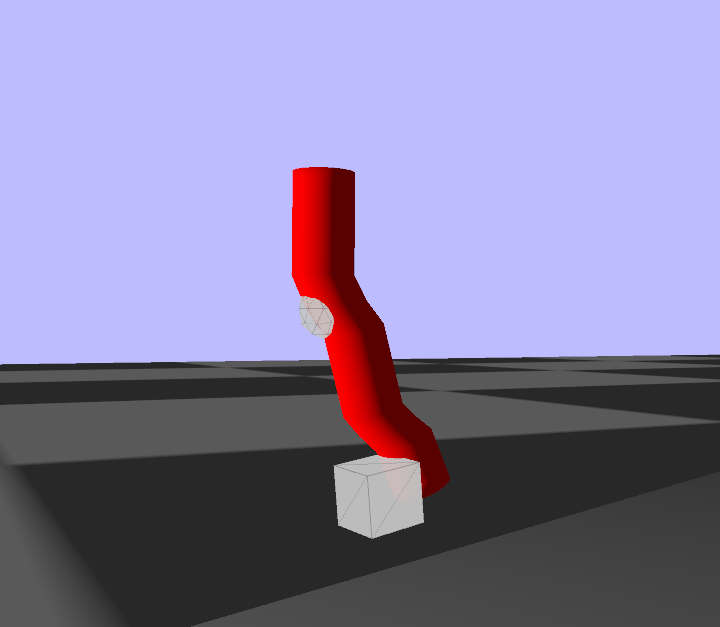
\includegraphics[width=0.8\linewidth]{softbody}
	\caption{Example soft body simulation. The grey objects with black wireframes are visualizations of rigid bodies used for debugging. The red deformed cylinder is driven by skeletal animation.}
	\label{fig:softbody}
\end{figure}

Figure~\ref{fig:fabric} shows cloth simulation. The model consists of \(32 \times 32 \) rigid bodies, and the solution of the constraint system took 111 ms per frame. In contrast, Figure~\ref{fig:pbd} shows a capture from our position-based dynamics implementation for cloth simulation using the same number of points, but only taking 1 ms per frame. While the PBD algorithm is much faster, it supports less features, and does not integrate seamlessly with classical rigid body simulations.

\begin{figure}[ht]
	\centering
	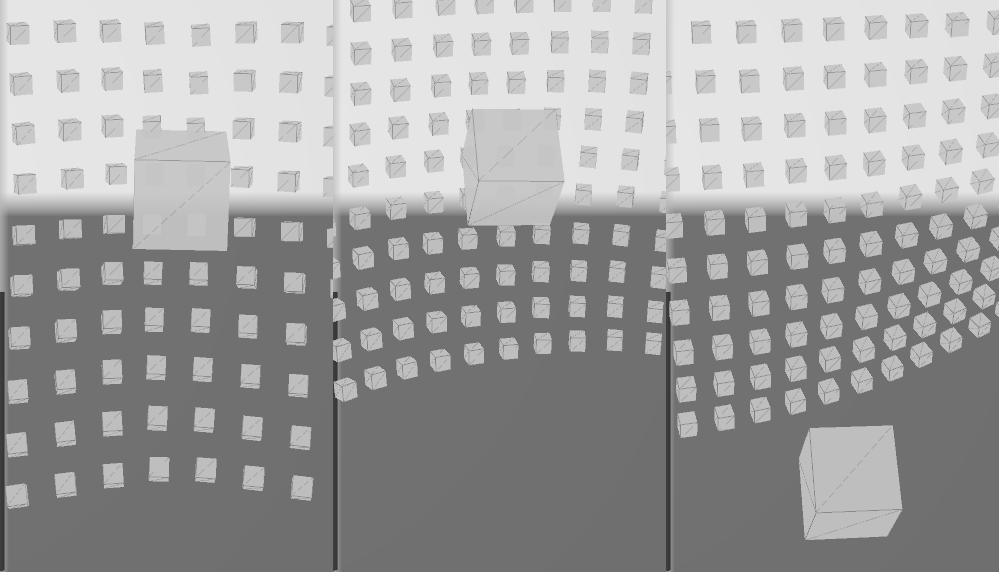
\includegraphics[width=0.8\linewidth]{sequence}
	\caption{Visualization of a fabric deformed after collision with a cube.}
	\label{fig:fabric}
\end{figure}

\begin{figure}[ht]
	\centering
	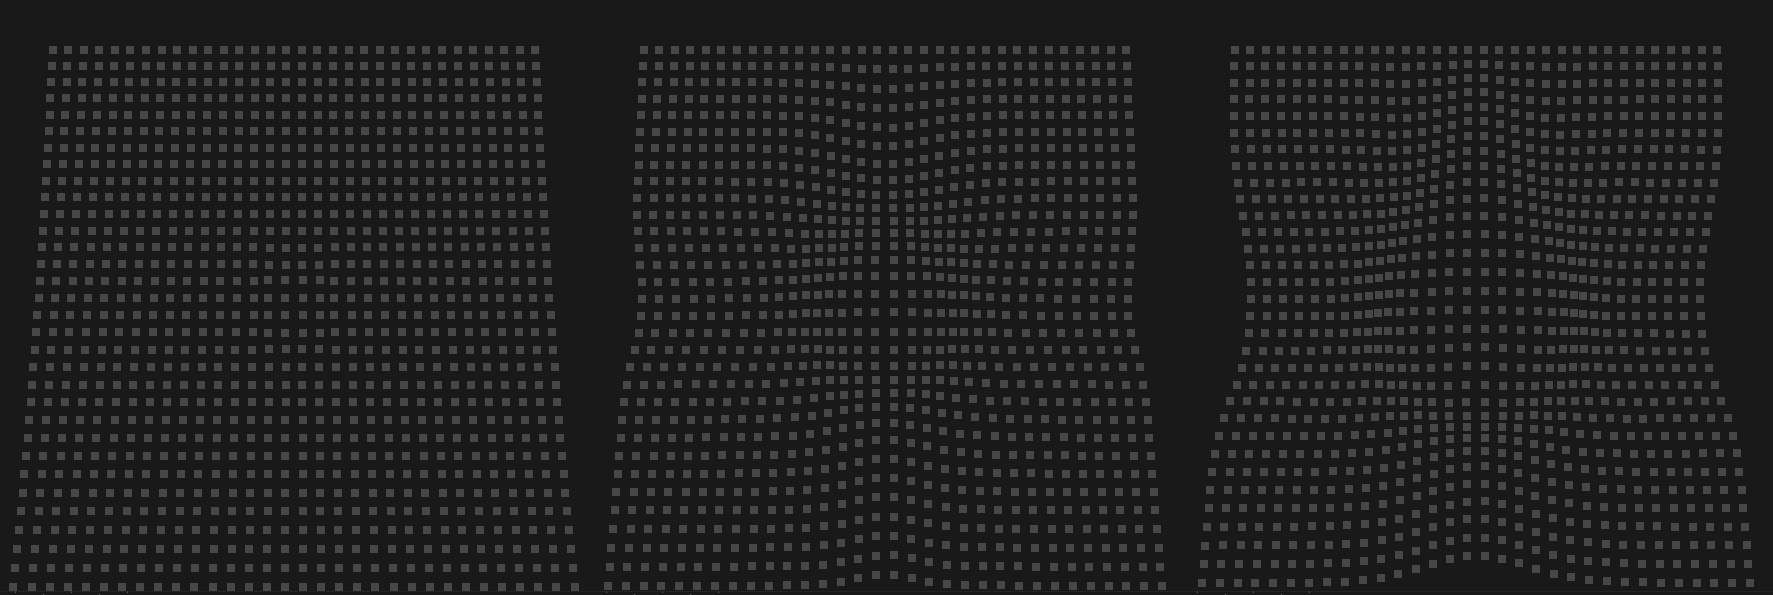
\includegraphics[width=0.8\linewidth]{pbd}
	\caption{Baseline PBD simulation.}
	\label{fig:pbd}
\end{figure}

\begin{figure}[ht]
	\centering
	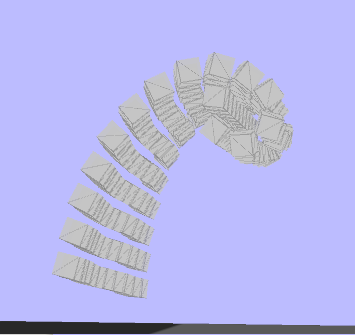
\includegraphics[width=0.8\linewidth]{roll}
	\caption{A sheet of fabric being rolled up.}
	\label{fig:roll}
\end{figure}

In Figure~\ref{fig:3d} three-dimensional soft-body simulation is illustrated. For 125 rigid bodies connected by 300 constraints, the solver took 13 ms per time step.

\begin{figure}[ht]
	\centering
	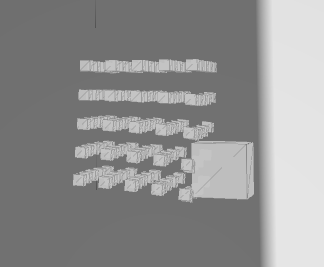
\includegraphics[width=0.8\linewidth]{3d}
	\caption{A three dimensional soft body deformed after collision with a cube.}
	\label{fig:3d}
\end{figure}

\begin{figure}[ht]
	\centering
	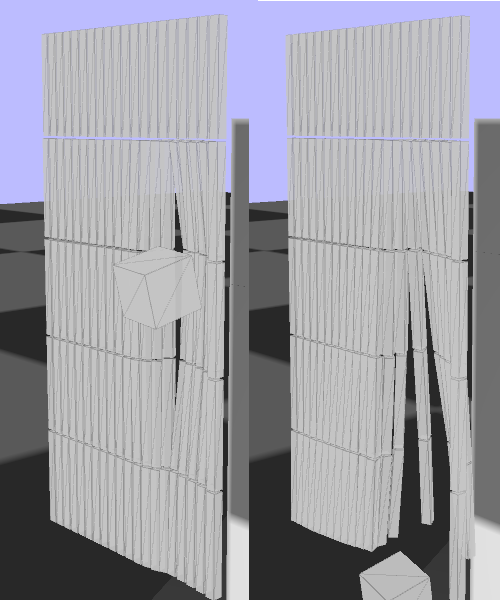
\includegraphics[width=0.8\linewidth]{rigid_hair}
	\caption{Hair simulation with rigid bodies.}
	\label{fig:rigid_hair}
\end{figure}

\begin{figure}[ht]
	\centering
	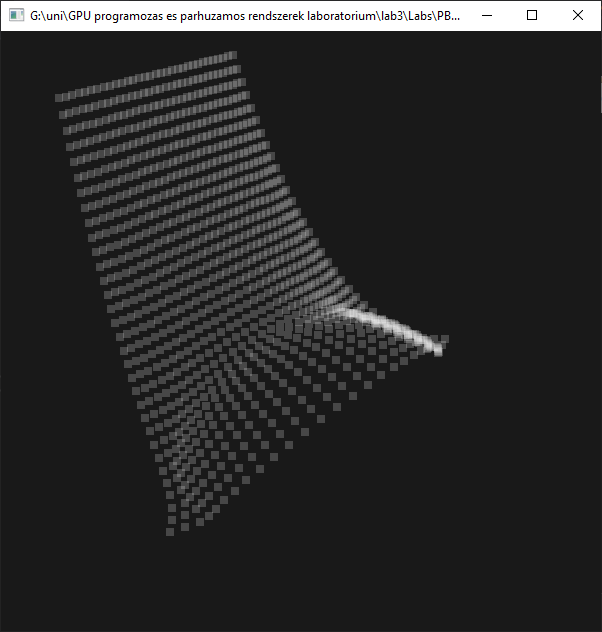
\includegraphics[width=0.8\linewidth]{pbd_hair}
	\caption{Hair simulation with PBD.}
	\label{fig:pbd_hair}
\end{figure}

\section{Conclusion}

Our measurements show that rigid-body simulation with generic constraints can achieve interactive performance even for relatively large element and constraint counts, realizing complex dynamic models. However, position-based solutions vastly outperform this approach. Therefore, rigid body simulations are only warranted if exact control over rotational constraints or collisions are needed, as is the case with physically animated skeletal ragdoll models. 

On current consumer devices, real-time simulation can only provide approximate results. While these are unsuitable for most engineering purposes, there are many applications in physics assisted 3d modeling, visualizations (conventional or VR), and video games.
 %%% The bibliography
\bibliographystyle{plainurl}
\bibliography{p}

\end{document}

\endinput
%%
%% End of file `cescgsmpl.tex'.
